\chapter{Architectural Design}

\section{Overview}
We chose to design the Students\&Companies (S\&C) web application using a three-tier architecture with remote presentation. These three tier correspond to a client tier, application tier and data tier. The client (presentation) tier serves the needs of both students, companies and universities using the S\&C platform. The application layer is the one that processes user request, performs statistical analysis and interacts with the internal data tier. The data tier is responsible for data management and storage. It handles all database operations, including data retrieval, updates, and management. To better improve and ensure load distribution and scalability, it was chosen to implement a load balancer between the client and application layer, in particular inside the web server.

A 3-tier architecture is suitable for a career service application as it makes the system easier to manage and scale. It ensures reliability through load balancing, which helps handle high traffic during peak usage. This architecture supports advanced features like job matching and analytics, integrates well with cloud services, and provides flexibility for future updates, such as adding mobile apps or AI tools. Its structure also improves security by isolating sensitive data in the database layer.

The S\&C architecture specializes in three different groups of components each with its own characteristics and responsibilities:
\begin{enumerate}
    \item Presentation layer: The Presentation (client) Tier is the application's front end, managing the user interface and interactions for data input and display. Its goal is to display data, collect inputs and provide a seamless user experience. 
    \item Application layer: It handles tasks like user authentication, recommendation matching algorithms, managing user accounts, handling notifications, and communication between the user interface and the database.
    \item Data layer: Stores and manages critical data such as user profiles, student's CVs, project descriptions, and application history. It ensures data security and efficient retrieval for real-time use in the application.
\end{enumerate}

\begin{figure}[H]
    \centering
    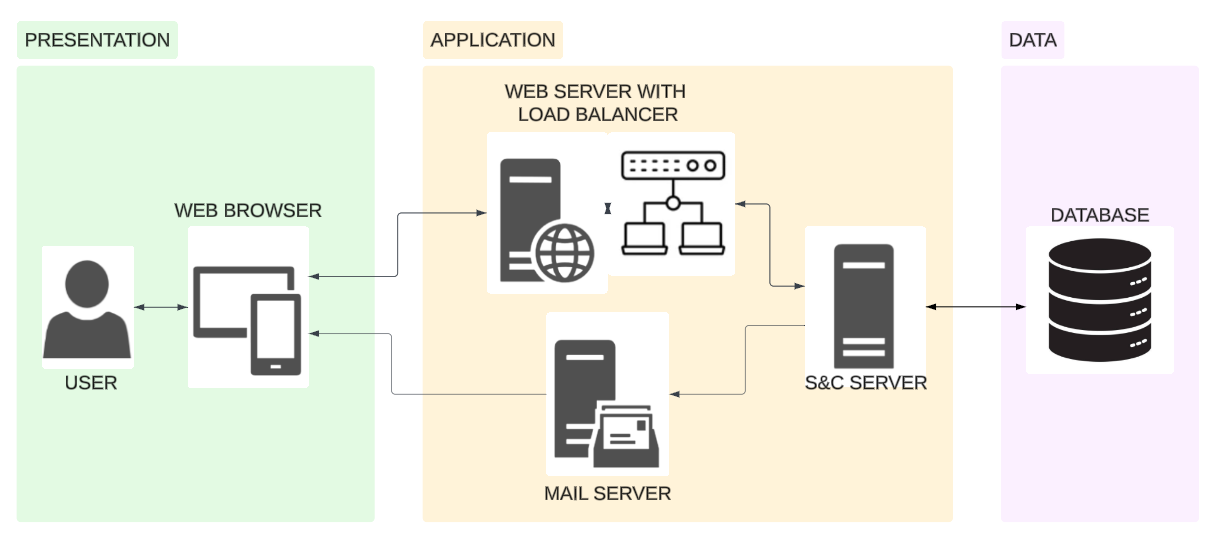
\includegraphics[width=0.8\linewidth]{DD//Images/3tier.png}
    \caption{High level architecture }
\end{figure}

\section{Component view} 

\subsection{Component diagram}

\subsection{Class diagram}
In this section, it is reported the class diagram, which has been already analyzed in the RASD document. 

(dopo aver definito tutte le component interfaces dovremmo rifare il class diagram con tutti i metodi definiti)

\begin{figure}[H]
    \centering
    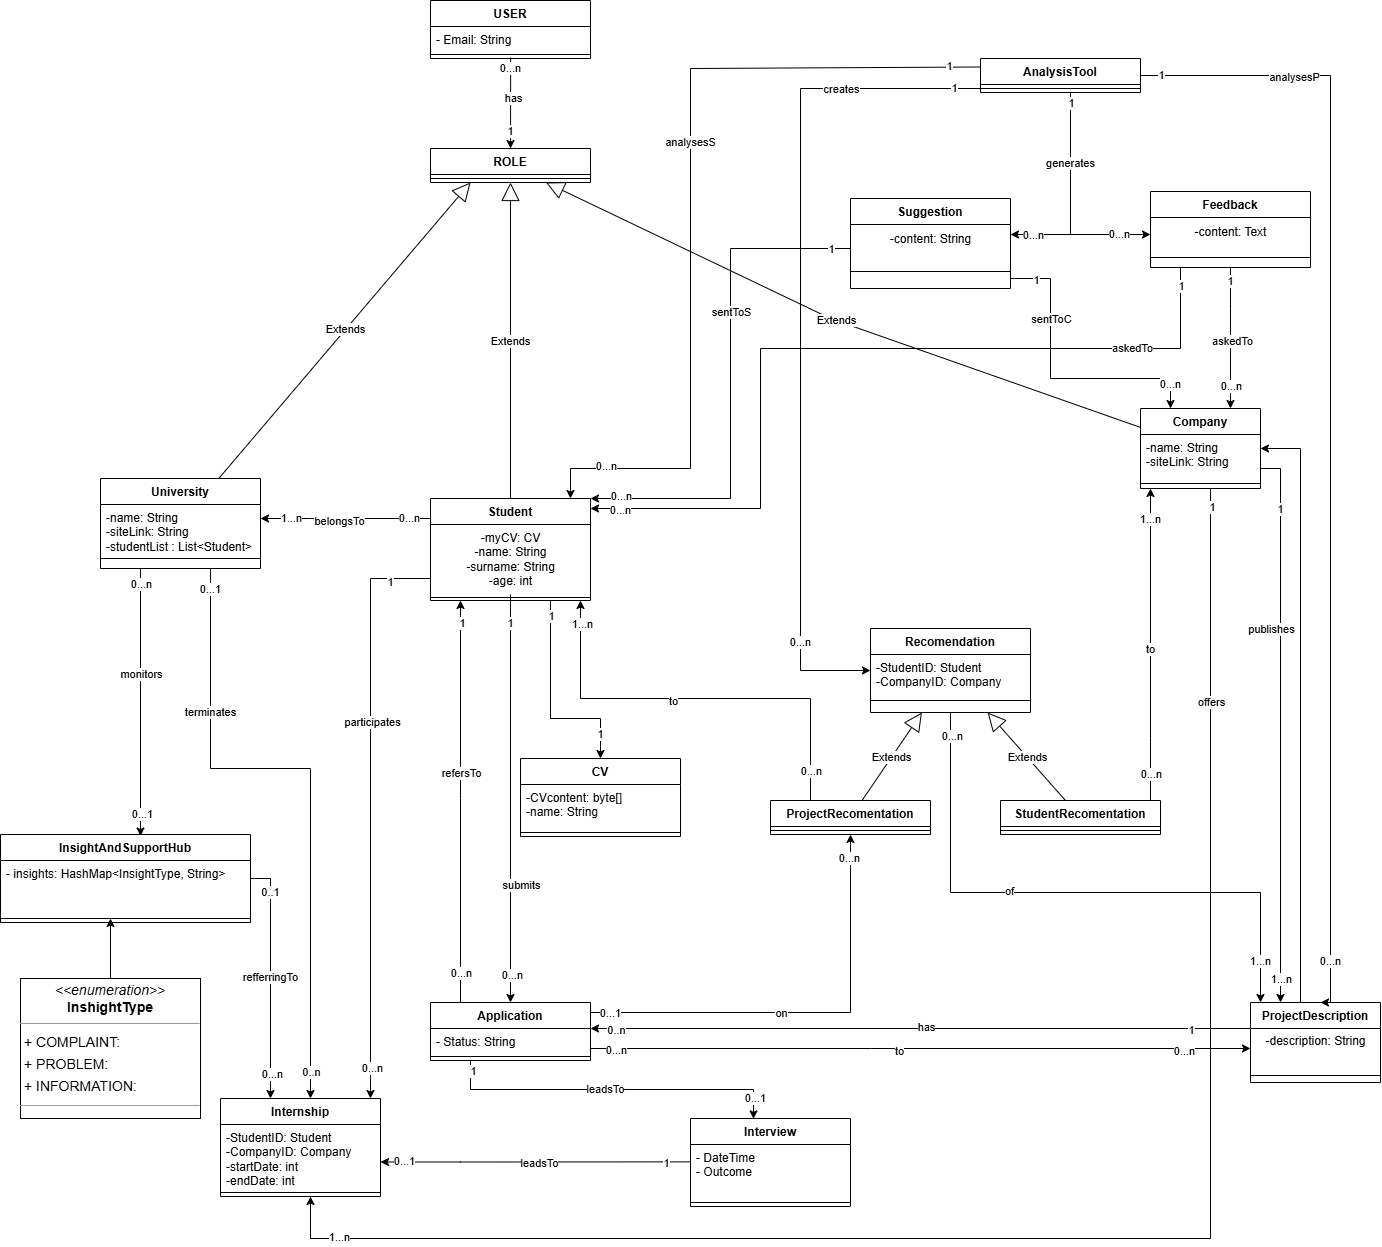
\includegraphics[width=1\linewidth]{RASD//Images/UML.drawio.png}
    \caption{Class Diagram }
\end{figure}


\section{Deployment view}

\section{Runtime view}

All the sequence diagrams described in the Requirements Analysis and Specification Document (RASD) will be elaborated in greater detail. In this expanded version, we will identify and specify the individual components of the application that are utilized to fulfill each specific functionality. 

Here below we will include an explanation of how each application component contributes to the implementation of the corresponding functionality. By doing so, we hope to provide a clearer understanding of the interaction between various components and their roles in achieving the described features and requirements.

Spiegazione su di cosa si occupa ogni component e poi tutti i sequence diagram..

\section{Component interfaces}
Tutte le interfacce (inserite nei vari diagrammi) e i loro metodi

\section{Selected architectural styles and patterns}
\section{Other design decisions }
